\chapter{Extremal Principle and Pigeonhole Principle}% by Nishat Anjum Bristy}

\begin{linkb}
   \begin{itemize}
        \item \href{https://www.youtube.com/watch?v=cYTssF84f9g}{Extremal and PHP (Bristy)}
        \item \href{https://drive.google.com/file/d/1sSvTee9gw9lAKwC0n6vyik79VrKpIiv6/view}{1}, \href{https://drive.google.com/file/d/17ps5RJ-FABW7CiSIj87zjC9de9FJyfn-/view}{2}, \href{https://drive.google.com/file/d/1_fbjgE7eFvVpFKNljJS24cN8NbPklCJu/view}{3}
   \end{itemize}
\end{linkb}

\section{Extreme Principle}
Every finite set has a least value and a greatest value. This is the basis of extreme principle.

As an example $\NN$ has the least value $1$.

Here is a motivating example of how to use extreme principle in Problem Solving.

\begin{example}
$n$ students are sitting in a field such 
that the distance between each pair of 
students is distinct. each student is 
holding a ball. When the teacher whistle, 
students throw their ball to the nearest 
student. Prove that there is a pair of 
students that throws their ball to each 
other.
\end{example}
Here starting with small values of $n$, we may guess the solution. The main idea is finding the least distance between two students. By extereme principle, there is a least distance betweeen two students. So, this $2$  students throw their balls to each other. Done!


\begin{example}
Find all the possible positive solutions to the equations.
\begin{align*}
x_1 + x_2 &= x_3 ^2 \\
x_2 + x_3 &= x_4 ^2 \\
x_3 + x_4 &= x_5 ^2 \\
x_4 + x_5 &= x_1 ^2 \\
x_5 + x_1 &= x_2 ^2
\end{align*}
\end{example}
Here you should guess the solution. You will find that $x_1=x_2=x_3=x_4=x_5=2$.

We will show that the solution must be equal to $2$, it can't be less that or grater that $2$.

By extremal principle, WLOG assume, $x_2$ is the least value here. So, we have,
\[ x_1 \le x_2, x_3, x_4, x_5\]
\[ x_1 \le x_4\]
\[ x_1 \le x_5\]
So, \[ 2x_1 \le x_4 +x_5 = x_1 ^2 \]
\[\implies x_1 \ge 2 \]

Similarly we can assume that $x_2$ is the greatest value here, and show that $x_2 \le 2$.

Then by the same argument, $x_3=x_4=x_5=x_1=x_2=2$.

So we are done.

\begin{example}
There are $n$ red points and $n$ blue points in a plane such that no three are collinear. Show that we can choose $n$  line segments so that, every line segment connects a red point with a blue point and no two line intersect . 
\end{example}
First, start with small values of $n$, you can find a monovariant here, that, if there is no intersections, then the sum of the lengths of the segments is least(by triangle inequality).

Let, assume a configuration with some intersections. Then, select an intersection, and then un-intersect it. In this process, we care about the sum of the lengths of the segments, by triangle inequality you can easily show that, with 4 points, if they intersects(2 line segments) then, in-intersect it and measure the sum, you can show that the last sum is obviously lesser than the previous.

It some point the sum become least. So we have to show that there is no intersection. Assume there is an inersection. Then using triangle inequality, there is a configuration with lesser sum, but we assumed the sum is least here. Contradiction!


\begin{example}
A finite set of points $S$ in a plane has the property that triangle determined by any thrree points in $S$ has area at most $1.$ Prove that, there exists a triangle with area $4$ that contains all the points
\end{example}
I am giving the solution with a diagram. :D 
\begin{figure}[h!]
\centering
	\includegraphics{php-tri.pdf}
	\caption{Guess the solution}
\end{figure}
%dont work


\section{Pigeonhole Principle}
Suppose there are $n$ pigeons to be placed within $n_1$ holes. Then you can easily say that there is hole which contains two pigeons. It is a trivial but very useful idea in solving combinatorial problems.
\begin{example}
A box has three pair of shocks colored red, blue and green. If the shocks are choosen without looking, at least how many shocks must be chosen to gurantee that at least one matching pair is there?
\end{example}
The answer is FOUR.


\begin{example}
Show that given a set of $n$ positive integers, there exists a non-empty subset where the sum of the elements is divisible by $n$.
\end{example}
Let, the set is $S=\{a_1, a_2, a_3, \dots , a_n \}$
And consider the following: 
\begin{align*}
s_1 &= a_1  \\
s_2 &= a_1+ a_2 \\
s_3 &= a_1, a_2, a_3 \\
\ldots \\
s_n &= a_1+ a_2+ \ldots + a_n
\end{align*}

$s_1, s_2, \ldots, _n$ may leave $n$ distinct residue modulo $n$ then one of them is $0$, done.

But if there are some two $s_i, s_j$ for which $s_i\equiv s_j \pmod n$ and $i<j$ then we have $s_j-s_i$ divisible by $n$.
\begin{example}
$10$ points are placed within an equilateral triangle of side length one. Show that, there exists two points with distance at most $\frac{1}{3}$ apart.
\end{example}
Look at the diagram. You may find the solution!
\begin{figure}[h!]
\centering
	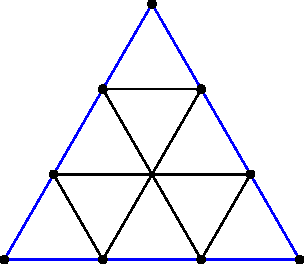
\includegraphics{php-tri-grid.pdf}
	\caption{There are nine triangle and ten points to be placed here!}
\end{figure}

Class ended!